The design of the \CaF{} chip experiment was motivated by three main factors:
the need to integrate with the existing experiment, the core proposal of
confining molecules close to a microwave guide, and the practicalities of
fabricating the chip. In this chapter I will describe how the first two factors
informed the design choices, with changes due to fabrication discussed in
chapter~\ref{fab}. The design will be further justified by simulation in
chapter~\ref{sim}.
%
We begin with a discussion of the existing experiment. I will then give an
overview and motivation of the design of the new experiment.


\section{Existing \CaF{} experiment}
\label{overview:existing}

In this section I will present a summary of the process used to produce
ultracold \CaF{} molecules in a magnetic trap, which we intend to load onto the
chip trap. We will consider the various stages of the process, which are
presented in \myfigref{overview:fig:CaFcartoon}. First a beam of \CaF{}
molecules is created using a buffer gas source~\cite{Truppe2018}. A fraction of
the molecules in the beam are slowed to below the capture velocity of the MOT
by radiation pressure from counter-propagating resonant
light~\cite{Truppe2017a}. We can also apply separate light in the transverse direction
to improve collimation of the beam during its flight.
The molecules are captured in a MOT~\cite{Williams2017} and cooled in optical
molasses~\cite{Truppe2017} before being optically pumped into a weak field
seeking state~\cite{WilliamsMagnetic2018}. This allows for magnetic trapping
and transport of the molecules. The experiment is conducted under ultra-high
vacuum (UHV, $P<\SI{1E-9}{\milli\bar}$) conditions to limit background induced
loss. Only the source chamber operates at a higher pressure, but the molecule
beam quickly exits this chamber into the low pressure region. 

\begin{figure}
  \centering
  \includegraphics[width=0.8\textwidth]{figs/overview/cartoon.pdf}
    %\begin{overpic}[width=0.8\textwidth]{figs/overview/cartoon_notext.pdf}
    %  \put(5, -1){Source}
    %  \put(32, -1){Slowing}
    %  \put(70.5, -1){MOT}
    %  \put(78, 55){\color{pink}{To chip}}
    %  \put(36, 52){\color{Lorange}{\pewpew{}{00} and repumps}}
    %  \put(95, 29){\color{Lgreen}{\pewpew{S}{00}}}
    %\end{overpic}
    %\vspace{1cm}
  \caption{A schematic of the \CaF{} source, slowing region and MOT chamber.
  \CaF{} molecules (blue) are produced by the buffer gas cell, and are
  slowed by longitudinal slowing and transverse cooling light (green,
  \pewpew{S}{00}). The molecules are then captured in a MOT (MOT light
  \pewpew{}{00} and repumps combined are shown here in orange) where
  they can be further cooled and transferred to a magnetic trap. The molecules
  can then be transported out of the chamber by the MTT in the direction of the
  pink arrow. A detailed view of the source is shown in
  \myfigref{overview:fig:source}}. This figure is based on one in
  \inlineref{Truppe2017}.
  \label{overview:fig:CaFcartoon}
\end{figure}

\subsection{\CaF{} energy structure and constants}

The energy structure of \CaF{} is depicted in
\myfigref{overview:fig:CaFenergy}. Here we show only the levels that are
pertinent to this thesis, those being the X, A and B electronic levels up to
vibrational level $v=3$, 2 and 0 respectively. The relevant Hund's cases are
(b), (a) and (b) respectively. For the X state, we will discuss $N=$
\numrange{0}{2} but for clarity $N=2$ is not included in this figure.
%
Figure~\ref{overview:fig:CaFenergy} and \mytableref{overview:table:lasers} also
label the various lasers that are used to addressed the \CaF{} transitions. We
denote these \pewpew{}{vv'} where $v$ ($v'$) is the lower (excited)
vibrational level that the laser addresses. The superscript $S$ is used to
distinguish the $X\rightarrow B$ transition.

\begin{figure}
  \centering
  % wide figure adds some padding to try and centre the levels a bit better
  \includegraphics[width=0.98\textwidth]{figs/energylevels/main_sbs_2_wide.pdf}
  \caption{
    The energy levels of \CaF{} are shown, along with the lasers that will be
    used to address the various transitions (further information is found in
    \mytableref{overview:table:lasers}). The branching ratios for the allowed
    decays are shown with dashed lines. Note that the $X(N=0)$ level is
    included, but for simplicity the $X(N=2)$ level is omitted. The box shows
    the hyperfine states of $X(N=1, v=0)$, and how these arise from the $N$ and
    $J$ angular momenta as described in the main text. This figure is adapted from
    \inlineref{Williams2017}. 
  }
  \label{overview:fig:CaFenergy}
\end{figure}

\begin{table}
  \centering
\begin{tabular}{llll}
  \hline\hline
  Symbol & Ground state & Excited state & Wavelength (\si{\nano\meter}) \\
  \hline
  \pewpew{}{00} & $X(v=0)$ & $A(v=0)$ &  606.3 \\
  \pewpew{S}{00} & $X(v=0)$ & $B(v=0)$ & 531.0 \\
  \pewpew{}{01} & $X(v=0)$ & $A(v=1)$ & 628.6 \\
  \pewpew{}{12} & $X(v=1)$ & $A(v=2)$ & 628.1 \\
  \pewpew{}{23} & $X(v=2)$ & $A(v=3)$ & 628.7 \\
  \pewpew{}{10} & $X(v=1)$ & $A(v=0)$ & 585.4 \\
 \hline
\end{tabular}
\caption{
  The various laser transitions used in this thesis.  The laser \pewpew{}{10}
  is included for completion, and will be explained in
  chapter~\ref{experiment}.
  }
  \label{overview:table:lasers}
\end{table}

The permitted decay paths are shown by the dashed lines, along with their
branching ratios. One of the reasons \CaF{} is chosen for study over other
molecules is its highly diagonal Franck-Condon factors, so that most decays
occur with $v'=v$. However, as we discussed in section~\ref{thoery:coolmols},
for large numbers of scattered photons we must employ the various repump lasers
to avoid pumping into states that are dark to the cooling light. This will be
discussed further when describing slowing of the beam and the MOT.

Hyperfine splitting occurs in \CaF{} due to the spin-half contribution of the
fluorine atom. This is not resolved in the $A$ state, but we account for the
hyperfine splitting of the $X$ state, which is shown in the box of
\myfigref{overview:fig:CaFenergy}. It worth explaining why we have the four $F$
states $F=2,1^+,0,1^-$. These arise due to an $\mathbf{S}\cdot\mathbf{N}$ term
in the Hamiltonian~\cite{}. Since we are in Hund's (b) case, the $N=1$ state is
split into angular momenta states $\mathbf{J}= \mathbf{N} + \mathbf{S}$. Here
$S=1/2$, so the possible values of $J$ are $3/2$ and $1/2$. Each of these is
again split by the hyperfine interaction into $\mathbf{F} = \mathbf{J} +
\mathbf{I}$, with $I=1/2$. This gives us the allowed values $F=2,1^+,0,1^-$.

In the $B$ level, the $F=0$ and $F=1$ states
are split by \SI{20}{\mega\hertz}, which can be neglected for the purposes of
our discussion. A full description of the \CaF{} energy structure and various
constants can be found in \inlineref{Anderegg2019a}, those that are most useful
are presented in \mytableref{overview:table:constants}.

\begin{table}
  \centering
\begin{tabular}{lll}
  \hline\hline
  Constant & Symbol & Value \\
  \hline
  Mass & m & \SI{59}{\amu}\\
  Electric dipole moment ($X$ state) & $\mu_e$ & $\SI{-3.08}{\debye}$\\
  % Don't confuse EDM with transition moment
  Magnetic dipole moment & $\mu_B$ & \SI{9.274}{\joule\per\tesla} \\
  % This is what Ed uses in his notebook, I think it is the same as mu_e...
  % Had to convert form his units, but pretty sure this is right.
  %Chemistry dipole moment & $\mu_c$ & $3\si{\debye}$ \\
 \hline
\end{tabular}
\caption{
  Various constants for \CaF{} taken from \inlineref{Anderegg2019a}. Note that
  the magnetic dipole moment is taken to be the Bohr magenton.
  }
  \label{overview:table:constants}
\end{table}

\subsection{Buffer gas source}

We begin all our experiments by creating a pulsed beam of \CaF{} molecules
using a buffer gas source. This is pictured in \myfigref{overview:fig:source}
and consists of a copper cell cooled to \SI{4}{\kelvin}. inside which the
\CaF{} molecules are formed from the reaction of \Ca{} atoms, ablated from a
target (shown in blue) by a Nd:YAG laser and \SFsix{} gas. Since the reagents
are hot (ablation warms the \Ca{} and the \SFsix{} is at \SI{270}{\kelvin}) it
is necessary to thermalise the molecules to reduce their temperature. This is
achieved with the eponymous buffer gas, in this case \He{}, which flows into
the cell at \SI{4}{\kelvin} and thermliases with the molecules before they exit
the cell in a beam.

\begin{figure}
  \centering
  \includegraphics[width=0.6\textwidth]{figs/overview/cell.pdf}
  \caption{The buffer gas cell. Helium and \SFsix flow into the cell. \Ca{}
  atoms are ablated from a target (shown in blue) by a Nd:YAG laser. \CaF{} molecules are
formed which thermalise with the \He{} and a molecule beam exits from the aperture.}
  \label{overview:fig:source}
\end{figure}

The cell is designed to optimise the flow of \He{} so as to thermalise with
\CaF{} and guide it to the exit aperture without the creation of vortices,
where the molecules can be trapped~\cite{Truppe2018}. For this reason \He{}
enters from towards the rear of the cell at \SI{4}{\kelvin} and flows towards
the exit aperture.  The \Ca{} target is  mounted on a rotating stage, so that
when one region is depleted another can be targeted.

In order to prevent excess helium entering the slowing and MOT chambers, a
second aperture is positioned between the source and slowing chambers.
Differential pumping ensures that the slowing chamber remains at UHV. A
mechanical shutter at this aperture reduces the time that helium is able to
leave the source chamber to only the time when there is a pulse of \CaF{}. We
also use a copper shield, coated with coconut charcoal and cooled to
\SI{4}{\kelvin} as a helium absorber~\cite{doi:10.1116/1.574141}. This is
thermally cycled overnight when the source is not in use to avoid saturation.
As noted in \inlineref{Jurgilas2021}, this buffer gas source originally
produced up to \SI{5E10}{molecules/steradian} molecules in $X(N=1, v=0)$ with a
mean velocity of \SI{160}{\meter\per\second}~\cite{Truppe2018} but its
performance has degraded since the original report. As a result we now observe
\SIrange{50}{60}{\percent} lower MOT population than at the time
\inlineref{Williams2017} was published.

\subsection{Slowing the beam}

The buffer gas source produces a beam of molecules with mean forward velocity
\SI{160}{\meter\per\second} -- slower than for example, a supersonic
source~\cite{Mathavan2016} but they are still far above the capture velocity of
our MOT, which is $\approx\SI{10}{\meter\per\second}$. The beam's velocity can be
further reduced by radiation pressure due to a counter-propagating beam of
\pewpew{S}{00} slowing light. This is chirped to account for the change in
Doppler shift of the transition frequency as the molecules slow. The slowing
light is also combined with the \pewpew{}{10} repump light to avoid pumping
into the $X(v=1)$ state. To again account for Doppler shift during slowing, the
repump light is frequency broadened by \SI{300}{\mega\hertz} by a series of
three elecro-optic modulators.

% Time and final velocity according to Hannah's thesis
We apply the light for \SI{6}{\milli\second}, which slows over approximately
\SI{90}{\centi\meter} of travel from the buffer gas cell's exit aperture.
Linear chirps used in previous experiments have been used to slow the molecules
for loading into the MOT, as detailed in \inlineref{Williams2017}. Implementing an
exponential chirp originally proposed in \inlineref{Anderegg2019}  produced a
\SIrange{60}{80}{\percent} improvement in the number of molecules in the
MOT~\cite{Jurgilas2021}.

Slowing the beam has the undesirable effect of increasing the transverse
velocity of the molecules. This is due to the stochastic change in the
molecules' momentum as they emit photons isotropically. The change in
transverse velocity is $v_r\sqrt{N_\gamma/3}\sim\SI{0.4}{\meter\per\second}$,
where $N_\gamma \sim 10^4$ is the number of photons scattered during cooling,
and $v_r=\SI{1.27}{\centi\meter\per\second}$ is the recoil
velocity~\cite{Jurgilas2021}.  One method of reducing this effect is to focus
the combined light so as to converge towards the cell to reduce transverse
scattering~\cite{Truppe2017a}.

\subsection{Transverse cooling}

The transverse heating effect can be further reduced by applying slowing beams
in the transverse direction, also on the $X\rightarrow B$ transition, but this
time the light has the r.f.\ sidebands to address the $X$ hyperfine structure
rather than the slowing chirp. This collimates the molecule beam due to Doppler
cooling taking place in the transverse direction. This process occurs before
the slowing light is turned on, any molecules that are pumped into $X(v=1)$ can
be re-cycled by the \pewpew{}{10} repump that is combined with the slowing
light. The slowing procedure described above is carried out simultaneously,
providing the remixing of dark ground states and the $v=1$ repump light.
%
Scattering of light in the transverse direction can collimate the beam, and has
been shown to improve the population of the MOT by a factor of
$\sim3$~\cite{Jurgilas2021}.

\subsection{Capture in a MOT}
\label{overview:MOT}

We aim to capture molecules in a MOT positioned \SI{130}{\centi\meter} from the
cell's exit aperture inside a separate vacuum chamber. The MOT magnetic field
is provided by in-vacuum anti-Helmholtz coils and the MOT light is formed from
a single beam which is reflected along each axis before being retro-reflected
through the entire experiment to provide the restoring beams.
%
We described in section~\ref{theory:coolmols} that laser cooling and trapping of diatomic
molecules requires us to address three key differences to atomic systems. The
first is the repumping of the vibational levels, which we have already allueded
to for the slowing. We apply vibrational repumps (\pewpew{}{10}, \pewpew{}{21}
and \pewpew{}{32}) along with the main cooling light (\pewpew{}{00}), to avoid
populating the dark states.  All of these beams must have the r.f.\ sidebands
to address the hyperfine levels of the $X$ state (recall that the hyperfine
levels of $A$ are unresolved).

The second nuance is the rotational branching, which we avoid by cooling on the
$X(N=1) \rightarrow A(N=0)$ transition. This immediately leads to the third
nuance, which is the remixing of resulting dark states. 
%
The \CaF{} MOT is a type-II MOT~\cite{1367-2630-18-12-123017}, meaning that the
angular momentum of the excited state ($A(v=0)$, with $F'=1$) is less than that
of the ground state ($X(v=0)$ with $F=2$). Unlike a type-I MOT (where $F'>F$),
it is therefore possible for a molecule that has been pumped into the excited
state to decay into a dark state, or into a state that is anti-trapped by the
MOT~\cite{Fitch2021}.
%
To resolve this, we employ a dual-frequency MOT. The main MOT transition is
addressed by the \pewpew{}{00} light, with r.f.\ sidebands added to address the
different hyperfine levels. The sideband addressing the $F=1$ hyperfine state
is given opposite polarisation, and simultaneously serves as a second frequency
for the $F=2$ state. This ensures that the normally anti-trapped states are
repumped by the restoring beam into the MOT cycle. The $F=2$ level is now
strongly trapped and although the other levels remain weakly trapped, this is
sufficient to create a strong MOT.

A simplified case with $F=0$ and $F'=1$ is shown in
\myfigref{overview:fig:dualfreq}. When there is no blue-detuned light, any
molecule that decays into the $m_F=-1$ state can be lost from the cycle. When
the blue-detuned light is present these molecules can be repumped. Since this
transition has a change in $m_F$ of $\Delta m_F = m'_F- m_F=1$, we require the
blue-detuned light to have $\sigma_+$ polarisation.

\begin{figure}
  \centering
    \begin{overpic}[abs, width=0.2\textwidth]{figs/overview/typeII.pdf}
      \put(-40, 43){$F=1$}
      \put(-40, 148){$F'=0$}
      \put(90, 43){$m_F=0$}
      \put(90, 81){$m_F=1$}
      \put(90, 5){$m_F=-1$}
      \put(5, 5){\color{blue}{$\sigma^+$}}
      \put(5, 81){\color{pink}{$\sigma^-$}}
    \end{overpic}
  \caption{
    A dual frequency scheme for the type-II case $F'=0$, $F=1$. The molecules
    in each state (circles) can be pumped by their corresponding red- (blue-)
    detuned light. This figure is adapted from one in \inlineref{Williams2018}.
  }
  \label{overview:fig:dualfreq}
\end{figure}

We are typically able to capture on the order of $10^4$ molecules from our
beam.  The MOT population can be estimated by the light-induced fluorescence.
The MOT temperature is reduced to its minimum value by lowering the intensity
of \pewpew{}{00}, since this reduces the effects of sub-Doppler
heating~\cite{Truppe2017}. We typically observe MOT temperatures of
$<\SI{4}{\milli\kelvin}$.
%
A complete description of the \CaF{} MOT is far beyond the scope of this
overview, and has been described in detail elsewhere, for example see
\inlineref{Williams2017}. We will not discuss an important alternative scheme
for forming a \CaF{} MOT, the r.f.\ MOT, a description of which can be found in
\inlineref{PhysRevLett.119.103201}.

\subsection{Optical molasses}

Sub-Doppler cooling of \CaF{} is achieved with a blue-detuned molasses. In this
scheme the MOT coils are switched off, and \pewpew{C}{00} is now blue-detuned
from the transition frequency. This scheme is somewhat complex, so consider
again the simplified example of a $F=1$ hyperfine level ground state, and $F=0$
excited state travelling in 1D, as is shown in
\myfigref{overview:fig:molasses}.  The counter-propagating beams establish a
polarisation-gradient, which couple the hyperfine states in $F=1$ to the $F'=0$
state. As explained in \inlineref{Weidem_ller_1994} we will have bright states
(superposition states of $\ket{F=1, m_F=1}$ and $\ket{F=1, m_F=-1}$) that are
coupled to the excited state by the a.c.\  Stark shift, and dark states
($\ket{F=1, m_F=0}$ and another superposition state) that are not coupled. The
strength of this coupling varies as a function of the polarisation, and so as
molecules move through the gradient the bright state energy changes, as is
shown in the figure.

\begin{figure}[htb]
  \centering
    \begin{overpic}[width=0.6\textwidth]{figs/overview/molasses.pdf}
      \put(-16, 82){$F'=0$}
      \put(-16, 30){$F=1$}
      \put(105, 19){Dark states}
      \put(105, 5){Polarisation}
      \put(105, 38){Bright states}
    \end{overpic}
    \vspace{1cm}
  \caption{Blue detuned molasses for a type-II system with $F=1$, $F'=0$. Here
    the polarisation gradient across a 1D system (bottom row) causes a change
    in the coupling strength of bright states. A molecule travelling through
    the gradient (blue) will be preferentially excited by \pewpew{}{00} to the
    excited state when the coupling is strong. It will decay into the dark
    states, and adiabatically transfer back to the light states (black arrow)
    when the coupling is weak.  Repeating this process results in a net loss of
  energy for the molecule. This figure is adapted from \inlineref{1367-2630-18-12-123017}.}
  \label{overview:fig:molasses}
\end{figure}

When a molecule in a bright state moves through the polarisation gradient it
can expend energy climbing the potential. At the top of the potential it is
preferentially pumped into the dark state via the excited state. From the dark
state, molecules can adiabatically transfer back into the dark state at regions
where the energy difference is low. The molecule can now repeat this cycle,
each time losing energy travelling up the potential. Note that the light must
be blue-detuned because in the case of red-detuning the bright states have
lower energy than the dark states, and there is a heating rather than a cooling
effect~\cite{1367-2630-18-12-123017}.

In the three-dimensional case the same principle applies but we must account
for intensity gradients, which will affect the change in coupling of the states
as well as polarisation gradients. We must also consider the numerous energy
levels of \CaF{} and the sideband structure required to address the hyperfine
state, a full treatment requires solving the optical Bloch equations, which is
done in \inlineref{1367-2630-18-12-123017}. In our experiment we apply this
technique to produce a \CaF{} cloud of temperature
$<\SI{6}{\micro\kelvin}$~\cite{PhysRevLett.123.033202}.

\subsection{Magnetic trapping and transport}

The molecules can now be transferred into a weak-field seeking state by optical
pumping. The weak-field seekers can be confined in a magnetic trap, provided
either by the MOT coils, or by the external transport coils. In the case of the
latter, the molecules can then be transferred to the tweezer chamber, or in the
future to the chip for loading.

During the molasses there is no magnetic field to lift the degeneracy between
the Zeeman states. Therefore after the molasses light is turned off the
molecules are distributed between the Zeeman substates of $X(v=0, N=1)$.
Attempting to magnetically trap at this point would cause a significant loss,
so we optically pump into the weak-field seeking state by a procedure originally
proposed for \SrF{} in \inlineref{PhysRevLett.121.013202} % this is Sarunas's ref 118
and described for \CaF{} in \inlineref{Jurgilas2021}.

In this scheme a weak magnetic field (\SI{200}{\milli\gauss}) is applied across
the cloud, and two beams of light are incident on the molecules. Both act on
the $X\rightarrow B$ transition, but their frequency components are tuned to be
close to the $F=2$ and $F=1^-$ hyperfine levels respectively. The $F=2$
($F=1^-$) frequency component propagates parallel (perpendicular) to the
magnetic field and its polarisation is chosen to drive $\sigma^+$ ($\pi$)
transitions. This means that the only state dark to the light is the
magnetically trappable state $\ket{N=1, F=2, m_F=2}$, which is eventually
populated. From here it is possible to transfer to other states by microwave
spectroscopy techniques~\cite{WilliamsMagnetic2018}. Various weak-field seeking
states of \CaF{} are detailed in \myfigref{overview:fig:magtrapstates}.

\begin{figure}
  \centering
  \includegraphics[height=0.45\textwidth]{figs/energylevels/magsplit.pdf}
  \caption{Hyperfine strucutre of \CaF{} ground states. The stretched states
    are highlighted in blue, and other weak-field seekers are highlighted in
    pink. Adapted from \inlineref{WilliamsMagnetic2018}.}
  \label{overview:fig:magtrapstates}
\end{figure}


% Removed the rot notation here, I think this is being taken out everywhere...
% TODO Check that this is the case
At this stage we also introduce three stretched states in \CaF{}. These states
lie in the $X$ electronic level, and are denoted
%
\begin{equation}
  \ket{N}_\text{str} = \ket{N, m_N=N}\ket{S, m_S=S}\ket{I,m_I=I},
\end{equation}
%
where the degeneracy must be lifted by the application of an external magnetic
field, $m_X$ is then the projection of $X$ onto this field's axis. The
stretched states are of interest because they are not only weak-field seekers,
but the transitions between neighbouring stretched states
($\ket{N}_\text{str}\leftrightarrow\ket{N+1}_\text{str}$) are highly
insensitive to magnetic fields. Of particular note are, the
$\ket{0}_\text{str}\leftrightarrow\ket{1}_\text{str}$ ($\omega_0/(2\pi) =
\SI{20.5}{\giga\hertz}$) and
$\ket{1}_\text{str}\leftrightarrow\ket{2}_\text{str}$ ($\omega_0/(2\pi) =
\SI{41.1}{\giga\hertz}$) transitions observed in
\inlineref{PhysRevLett.124.063001}, which we will discuss further in
chapter~\ref{mws}.

After transferring into the magnetically-trappable states, the molecules can be
contained in a quadrupole magnetic trap, as also discussed in
\inlineref{WilliamsMagnetic2018}. We can transfer them to a magnetic transport
trap (MTT), where they can be transferred to neighbouring experiments, or we
can hold them in the field generated by the MOT coils for experiments in the
collisions chamber.

\subsection{Other experiments}

The \CaF{} MOT is the workhorse of our experiment, providing molecules which
can be further cooled cooled further (as discussed above) used for experiments
in collisions with \Rb{} atoms (see \inlinerefs{Jurgilas2021, JurgilasIOP2021,
PhysRevLett.126.153401}) and optical tweezers. The tweezer experiment is
undertaken in the neighbouring tweezer chamber, which is loaded by transporting
molecules in the MTT, a quadrupole trap with coils mounted on a transport stage
outside the vacuum chamber. This transport of the molecules is similar to that
used in \inlinerefs{Lewandowski2003,PhysRevResearch.1.033035} and elsewhere. It
will be discussed further in chapter~\ref{experiment}. In the next section, we
will begin to discuss how the molecule chip can also be incorporated as an
additional experiment.


\section{Design requirements and overview}
\label{overview:design}

As discussed in \cm{the introduction} the aim of this project is ultimately to
trap molecules in close proximity to microwave resonators so that we can
perform coherent control of quantum states on the rotational transitions in the
molecules.
%
Following the proposal by \inlineref{Andre2006}, this can be achieved in a chip
architecture, with the molecule trapped as close to the resonator as possible.
%
The limiting factor will come from the Van der Waals force, where the
fluctuating electric dipole moment of the molecule results in attraction
between the molecule and the chip surface~\cite{}. The associated energy
shift is 
%
\begin{equation}
  V_\text{vdW}(z) \approx \frac{\mu_e^2}{4\pi\epsilon_0 h z^3}.
\end{equation}
%
We want this and the gradient $V'_\text{vdW}(z)$ to be small compared to the
vacuum Rabi frequency found in \cm{reference theory section}. We find this to
be true when $z\geq\SI{10}{\micro\meter}$, which we deem is the closest that we
will trap molecules to the surface.  We therefore require that trapping
electronics will be on a smaller scale than this so that trapping potential is
sufficiently localised.  Features of such a size can be easily created by
standard photolithography techniques.

Additionally, we aim to integrate the chip trap into our existing \CaF{}
experiment. This can be done by the addition of a new chamber to our setup,
shown in \myfigref{overview:fig:vacuumsystem}. The chip chamber will be
positioned along the existing MTT axis, allowing extension of the transport
system and the delivery of molecules to this chamber. \CaF{} molecules can then
be transferred onto the chip trap.

\begin{figure}[htb]
  \centering
    \begin{tikzpicture}
      \node[anchor=south west,inner sep=0] (image)
{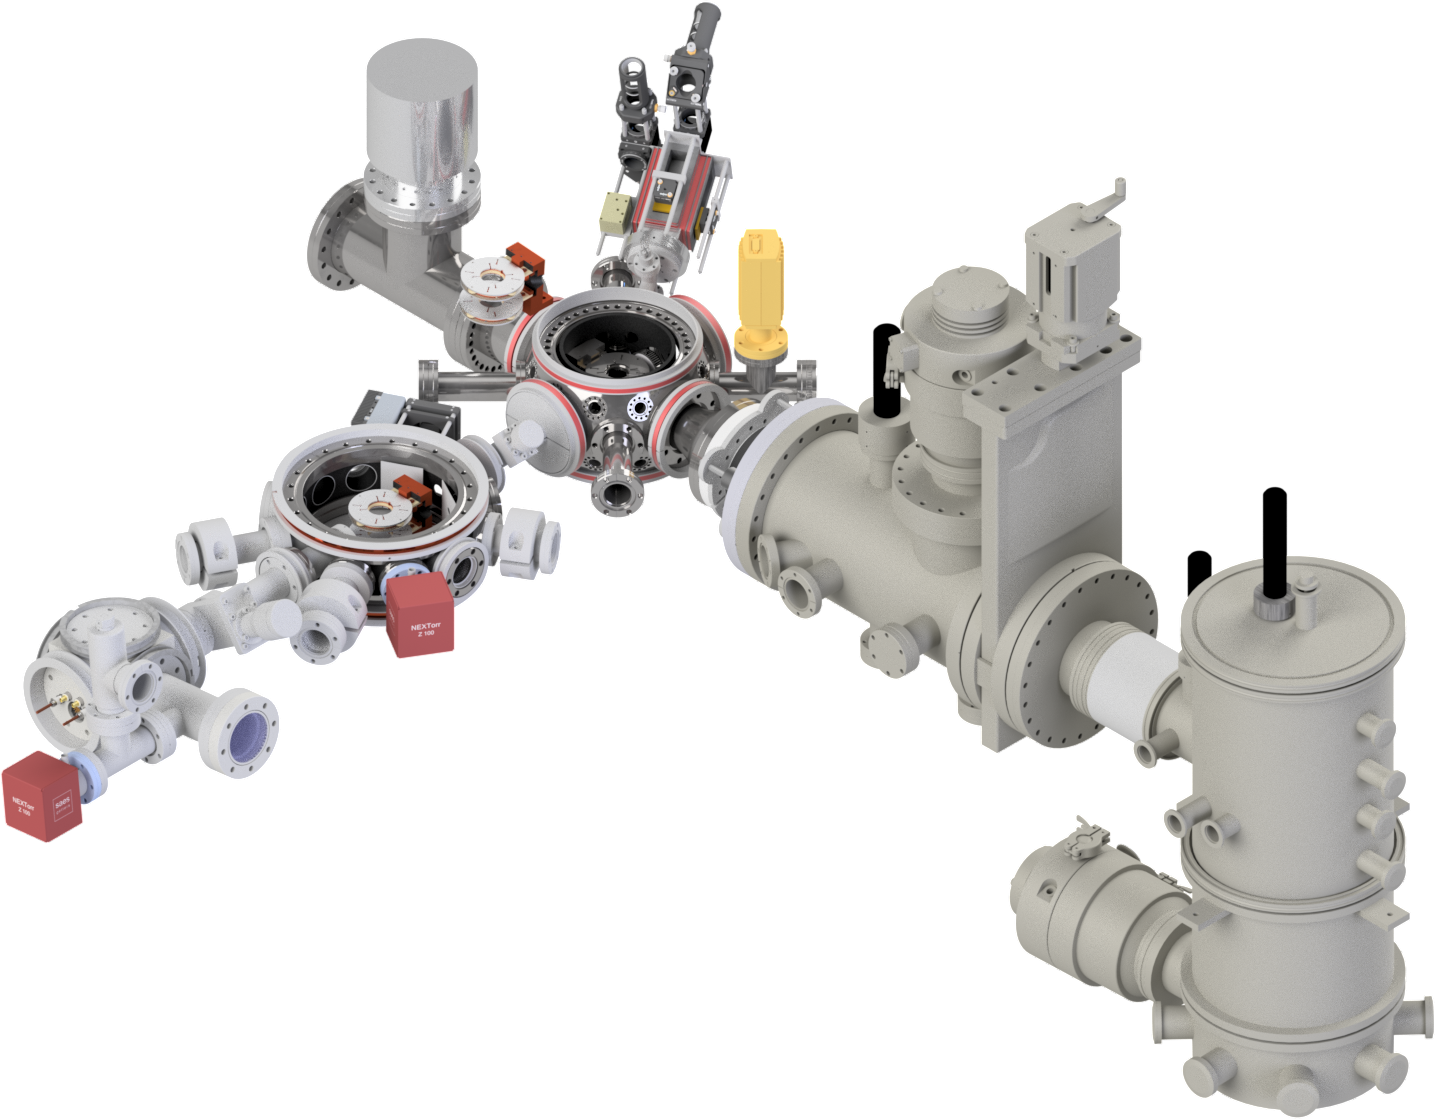
\includegraphics[width=0.8\textwidth]{figs/overview/apparatus_04_crp.png} };
      \begin{scope}[x={(image.south east)},y={(image.north west)}]
        \draw [-stealth] (0.45, 0.35) -- (0.45,0.52);
        \node[] at (0.46,0.3) {\small MOT chamber};
        \draw [-stealth] (0.18,0.23) -- (0.1, 0.3);
        \node[] at (0.21,0.2) {\small Chip chamber};
        \draw [-stealth] (0.15, 0.7) -- (0.2,0.63);
        \node[] at (0.12,0.72) {\small Tweezer chamer};
        \draw [-stealth] (0.7, 0.95) -- (0.52,0.85);
        \node[] at (0.72,0.99) {\small \Rb{} cell};
        \draw [-stealth] (0.95, 0.85) -- (0.8,0.7);
        \node[] at (0.97,0.89) {\small Slowing region};
        \draw [-stealth] (0.6, 0.2) -- (0.7,0.2);
        \node[] at (0.54,0.2) {\small Source};
      \end{scope}
    \end{tikzpicture}
  \caption{
    The \CaF{} experiment is shown along with the planned additional chip
    chamber. Not shown: external transport coils and transverse cooling region.}
  \label{overview:fig:vacuumsystem}
\end{figure}

At this point, we note that the long-lived stretched states discussed in
section~\ref{overview:existing} are promising candidates for the qubit states
in a molecule chip. For this reason it was decided that using magnetic traps,
such as those described in \cm{ref theory section} would be preferable to the
electrostatic traps suggested in \inlineref{Andre2006}. We are now faced with
the question of how exactly we can load molecules from the MTT into the
microscopic chip trap.

% TODO Check this para because I will presumably discuss relevant stuff in
% intro/theory
Fortunately this problem has previously been addressed for atom chips. We
discussed already in \cm{reference intro} that atoms can be guided on chips by
changing of trapping currents and voltages. We also discussed the transfer of
atoms between on-chip magnetic traps. For the problem of loading from a
macroscopic trap, we can turn to \inlineref{Ott2001}, where transfer from a
transport trap to a microtrap is made easier by the use of an intermediary
macroscopic trap that is well-aligned with the microtrap.
We propose a similar solution: embedding a mcaroscopic U-wire beneath our chip
trap which is aligned to the chip and makes a large target for loading form the
MTT.  This will be discussed further in \cm{experiment chapter}.

To ensure that molecules are then loaded into the smallest trap efficiently, we
again follow the footsteps of atom chips, and have designed  a series of traps
of decreasing size~\cite{Reichel1999}. For magnetic traps, the width of the
wires should decrease, so that the molecules remain localised around
the trap centre throughout loading. 
%
Each wire trap will begin trapping at one height before the bias field is
increased to bring the trap centre closer to the surface (as per
\myeqref{theory:eqn:height}). We choose the wires to be Z-traps so as to avoid
any losses by spin-flips, and so we label the stages $\mathrm{ZX_i}$ for
initial (higher) traps and $\mathrm{ZX_f}$ for the final (lower) trap, with
$\mathrm{ZX}$ corresponding to the wire labels in
\mytableref{overview:table:wires}. Bias fields for all traps are to be provided
by external Helmholtz coils.

Each Z-wire should be sufficiently large to maintain the currents required to
form a trap at height $z$ below the trap, whilst having a width and height  $w,
h \ll z$ so that that the current is highly localised compared to the cloud
size.
%
In the case of the first Z-wire, the molecules are still \SI{3}{\milli\meter}
away from the trapping wire. If we demand a trap depth of
$k_B\times\SI{1}{\milli\kelvin}$, then we require a trapping current of
\SI{30}{\ampere} to form a trap of this depth.  We will discuss in
chapter~\ref{fab} that the maximum wire height that can reliably be fabricated
is \SI{5}{\micro\meter}, and we expect that the wires will be able to carry a
maximum current density of \SI{6E10}{\ampere\per\meter\squared}, as was found
for a similar chip design in \inlineref{Treutlein2008}. The Z-wire will
have a width $w=\SI{200}{\micro\meter}$. The currents and widths of other wires
are calculated similarly.
%
All wires have been designed to
carry twice the current that is required in the loading scheme, so that there
is sufficient headroom for further experiments, and to reduce risk of
accidental damage to the chip during normal operation.
%
The axial length of the wires also decreases to gradually reduce the size of
the trapped cloud in the $x$ direction.  

\begin{table}
  \centering
\begin{tabular}{lrrrrr}
  \hline\hline
  Name & Axis length (\si{\milli\meter}) & Width (\si{\micro\meter})& $I_\text{max}$ & Trap height (\si{\micro\meter}) \\
 \hline
  U & 16 & N/A& 100 & 3000\\
  $\mathrm{Z0}$ & 12 & 200& 60& $3000\rightarrow1000$ \\
  $\mathrm{Z1}$ &  6 & 20& 6& $1000\rightarrow100$ \\
  $\mathrm{Z2}$ &  2 & 9& 2.7& $100\rightarrow10$ \\
 \hline
\end{tabular}
  \caption{Details on the wire dimensions, maximum current, and desired
  trapping heights. The wire design is shown in
  \mysubfigref{overview:fig:chiplayout}. Note that the U-wire current is
  limited by vacuum feedthroughs and not by the maximum current calculated by
  the wire dimensions.  The maximum currents have been designed for use at only
  50\% of their potential maximum ($I_\text{max}$).
  }
  \label{overview:table:wires}
\end{table}

The final chip design was informed both by the requirements here, the
simulations presented in chapter~\ref{sim} and the restrictions due to the
fabrication process, which will be discussed in chapter~\ref{fab}. We tried
various different designs, but the final one that was chosen is shown in
\myfigref{overview:fig:chiplayout}. It features the wires as stipulated in
\mytableref{overview:table:wires}, fanouts for connection of macroscopic
current delivery wires, and various other features that will also be explained
in chapter~\ref{fab}.

\begin{figure}[ht]
  \centering
    \begin{overpic}[abs, width=0.51\textwidth]{figs/chip_present4.pdf}
      \put(10, 160){\small (i)}
      \put(60, 160){\small(ii)}
      \put(175, 60){\small(iv)}
      \put(110, 137){\small(iii)}
      \put(70, 90){\small \SI{20}{\micro\meter}}
      \put(112, 93){\small\SI{10}{\micro\meter}}
      \put(8, 42){\small $\mathrm{Z_0}$}
      \put(8, 10){\small $\mathrm{Z_1}$}
      \put(8, 200){\small $\mathrm{Z_2}$}
    \end{overpic}
  \caption{
    A schematic of
    the chip features, with the scaling exaggerated for visibility. The three
    overlapping Z-wires are shown and labeled. The gaps between the wires are
    highlighted.
    %
    Toward the left (i) is the
    electroplating connection pad and various features used for
    characterisation (ii). On Z2 it is possible to see several small pads used
    as anchors, to secure the thin wire to the substrate.  The axis of the
    $\mathrm{Z1}$ wire is labeled for reference (iii) and the other wires are
    similar. All of the above features  will be discussed further in
    chapter~\ref{fab}. The crest of Imperial College London (iv) is also
    included.}
  \label{overview:fig:chiplayout}
\end{figure}

Notice that this design does not incorporate microwave guides. These are to be
installed on a second level, separated from the trapping wires by a thin
insulating layer, on which we can fabricate coplanar waveguides~\cite{1127105}.
This stage of the project has not yet been reached, but the planned fabrication
procedure for microwave guides is discussed in \cm{ref section} and their
operation is discussed in chapters~\ref{mws} and \ref{squeeze}.

\begin{figure}[htb]
    \centering
    \begin{tabular}[t]{c}
\begin{subfigure}{\textwidth}
    \centering
    \smallskip
    \begin{overpic}[abs,
      width=\textwidth]{figs/exper/labeled_explosion.pdf}
      \put(20, 132){(a)}
    \end{overpic}
\end{subfigure}
    \\[1cm]
        \begin{tabular}{cc}% if you add [t], than sub images are pushed down
        \smallskip
            \begin{subfigure}[t]{0.45\textwidth}
                \centering
                \begin{overpic}[abs, width=\textwidth]{figs/overview/chamber_xsecarrow.pdf}
                  \put(5, 160){(b)}
                \end{overpic}
              \end{subfigure}&
            \begin{subfigure}[t]{0.45\textwidth}
                \centering
                \begin{overpic}[abs, width=\textwidth]{figs/chip_pic_crop.png}
                  \put(1, 160){(c)}
                \end{overpic}
            \end{subfigure}
        \end{tabular}
    \end{tabular}
  \caption{
  The chip experiment is shown in detail. In (a) we show an exploded view of
  the chip flange assembly, with the various components labeled.
  A cross section of the chip chamber is shown in (b). The arrow shows how
  molecules will enter the chamber, brought in by the MTT.
  In (c) we have the chip assembly fully constructed, with a view of the
    aluminium-core PCB (subchip) for current delivery. The
    microwave feedthroughs remain disconnected.
  }
  \label{overview:fig:chipchamber}
\end{figure}

To facilitate all of this, the chip and supporting infrastructure is mounted on
a flange with supporting infrastructure, as detailed in
\myfigref{overview:fig:chipchamber}. This chip flange assembly is equipped with
a large copper heat sink, a large U-wire to form the macroscopic alignment trap
and a subchip for current and microwave delivery. It is mounted into a recess
in the subchip so that it is flush with the surface. The chip is mounted facing
downwards so that molecules can be dropped for imaging as they fall. The flange
itself is fitted with two high-current (\SI{100}{\ampere}) feedthroughs, a
16-pin feedthrough rated for \SI{3}{\ampere} currents, and microwave
feedthroughs. All access to the chip is therfore through this one flange,
allowing for easy access and assembly.  It will be housed in a separate vacuum
chamber (the chip chamber), positioned as shown in
\myfigref{overview:fig:vacuumsystem}. The chip chamber will be arranged so that
Molecules can be brought in along the transport axis (shown by the arrow in the
\mysubfigref{overview:fig:chipchamber}{b}) and positioned below the surface of
the chip.  This arrangement will be explained in further detail in
chapter~\ref{experiment}.
